\chapter[Results and future developments]{Results and future developments}

\section[Measurements summary]{Measurements summary}

\subsection[Input power levels]{Input power levels}

A number of measurements have been collected during 2016. Figure \ref{g_IP} shows the relation between the average gradient and the input power in the accelerating structure with the measurement points highlighted. The measurement points have been selected to allow the comparison between the different running conditions, as outlined in Chap. \ref{chap:motivation}, and are summarised in Table \ref{run_pwr}.

\begin{table}
  \centering
    \begin{tabular}{ c l }
    \hline
    \hline
    Run type		&	Input power (MW)		\\
    \hline
    unloaded 		&	43.3, 41, 38 and 24.6	\\
    loaded			&	43.3, 41 and 38			\\
    anti-loaded		&	6.5					\\
    \hline
    \hline
    \end{tabular}
\caption{Input power levels of measurements of 2016 measurement campaign.}
\label{run_pwr}
\end{table}

The measurements at different input power level have not been taken in a precise order, anyway it has been tried to keep long measurement periods as much as possible at the same input power. 
The choice is normally complicated by the fact that the Xbox was not able to provide the maximum RF power level during the year, mainly because of technical problems.


\subsubsection{Comparison of loaded and unloaded runs at same average gradient}

For the CLIC test purpose,  carry out a measurement at 100 MV/m average gradient comparing loaded and unloaded runs would be the most interesting measurement possible. In order to perform it, the input power has to raised from 43.3 MW in the unloaded case to 67.5 MW in the loaded case (with a beam current of 1.6 A). 

Unfortunately it was clear from the beginning that reaching 67.5 MW of input power was not possible because the waveguides that deliver the power from the pulse compressor to the structure under test are not conditioned for such high power flux.

Because of this limitation, the choice comes down to perform measurements at the same input power and compare the results. 

During a period of technical problems, it has been anyway collected an unloaded measurement at 24.6 MW of input power, in order to compare it with the correspondent average gradient in the loaded case at 43.3 MW of input power. Unfortunately with a such low input power, the breakdown rate is very low, and after 4 days of measurements zero breakdowns were collected. Therefore it is only possible to affirm that running unloaded at 24.6 MW input power, the breakdown rate is $< 7.7 \, 10^{-8} $ BD pulse$^{-1}$. 


\subsubsection{Comparison of loaded and unloaded conditions at same input power}

Most of the measurements carried out during 2016 campaign were comparing the loaded and unloaded running condition. The input power levels used were 43.3, 41 and 38 MW. It was not possible to go at lower input powers because the breakdown rates becomes so low that the data collection takes weeks to produce a sufficient statistics.


\subsubsection{Study of the antiloaded runs}

The antiloaded measurements were carried out at 6.5 MW of input power. The reason is that with a beam current  of 1.6 A, the output gradient of the structure is already around 100 MV/m (see Fig. \ref{3grad}). The results were indeed interesting and will be shown later when it comes to talk about the breakdown distribution.




\begin{figure}[t]
\centering 
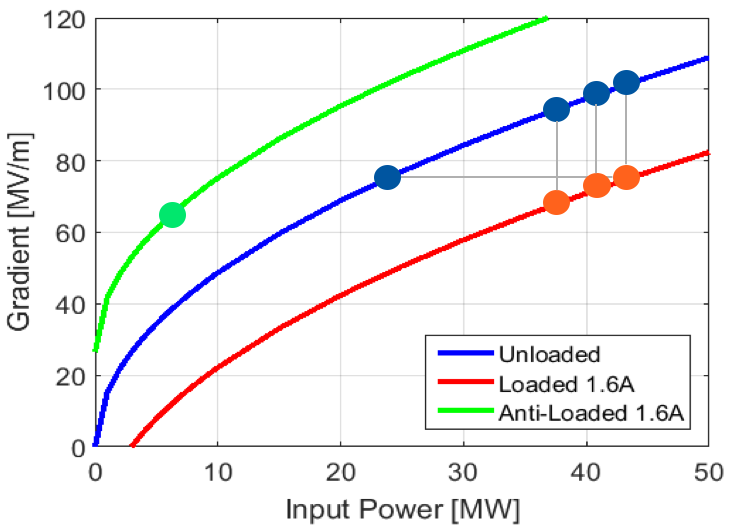
\includegraphics[scale=0.7]{pictures/grad_vs_inPow.png}
\caption{Average gradient as function of the input power in different running conditions. See text for details on the measurement points. }
\label{g_IP}
\end{figure}


\subsection[Beam pulse parameters]{Beam pulse parameters}

As mentioned in the motivation of the experiment, the goal is to understand the effect of the beam on the breakdown rate. The beam parameters have been therefore selected in order to enhance the effect of the beam, rather than try to simulate the CLIC operation. This materialises in:
\begin{itemize}
\item Higher beam current than CLIC: 1.6 A instead of 1.2 A.
\item Longer beam pulse: the beam is lasting during all the compressed RF pulse, lasting 250 ns, instead of last just during the flat-top of the CLIC pulse (see Sec. \ref{sec:PCtune}).
\end{itemize}

\noindent
The loaded operation is clearly visible  in the RF signals, as shown in Fig.~\ref{RF_load}.

\begin{figure}[h]
\centering
  \subfigure[Loaded operation]
   {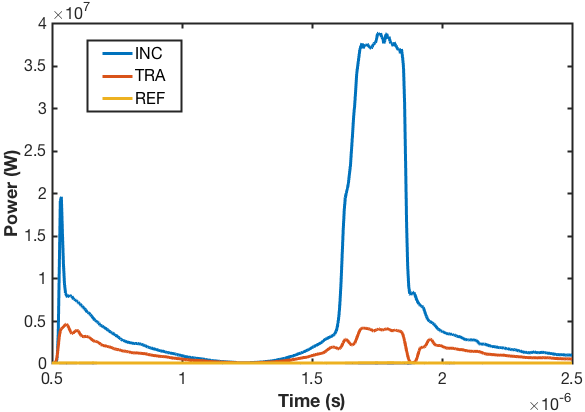
\includegraphics[scale=0.33]{pictures/LoadedPulse.png}}
  \subfigure[Antiloaded operation]
   {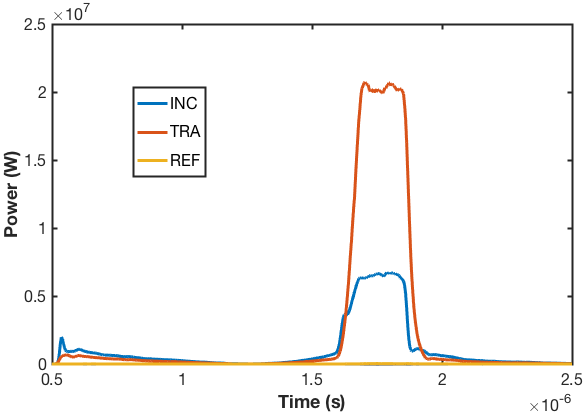
\includegraphics[scale=0.33]{pictures/AntiloadedPulse.png}}
\caption{Comparison of the RF signals during the loaded and antiloaded operation. During the loaded operation it can be observed that the transmitted power falls close to zero, because of the energy subtracted from the beam. The opposite behaviour can be noted in the antiloaded case, where the input power is much lower than the transmitted. In this case the difference in energy is provided by the beam, that gets slowed down because of the wrong phase with the RF. }
 \label{RF_load}
 \end{figure}



\section[Breakdown rate measurement results]{Breakdown rate measurement results}

The breakdown rate has been calculated per every run, as described in section \ref{sec:BDR} and is reported in Fig. \ref{BDR_history}. 

A fluctuation of the breakdown rate is appreciable. Considering separately unloaded or loaded runs data at the same input power, the excursion of the fluctuations is estimable as one order of magnitude. 

A weird behaviour is observed from July on, when the BDR raises for more than two months long, while running at 38 MW input power. It is possible that the antiloaded runs between June and July (plotted in green) have some effect on the overall BDR of the following runs. A similar variation of the breakdown rate is observable when changing the input power level of the structure.


\begin{landscape}

\begin{figure}
\centering 
\includegraphics[scale=0.62]{pictures/bdr_hist.png}
\caption{History plot of the measured breakdown rate.}
\label{BDR_history}
\end{figure}
 
\end{landscape}



In general breakdown rate measurements need stable running conditions, and a fluctuation of the BDR is appreciable also in the unloaded tests in the other Xboxes. Normal measuring times involve measuring periods of the order of weeks. In this experiment, the average stable running time was alternatively four days without beam and 2 days running with the beam (up to two half-days per week are normally lost in operation and down-time). It is not possible to foresee the impact of this on the breakdown rate. Considering that when changing the input power, the BDR seems to increase, it is reasonable assume that the accelerating cavity is a system that needs a settling time to stabilise. A similar process could take place when switching form operation with beam to without and vice versa. The reason is that even if the input power remains the same, the fields inside gets modified and the structure needs time to settle. 

A new insight on the effect of the input power switch will be given in the close future from the DC test stand at CERN, that has the possibility to acquire data much faster than any other RF-based experiment \cite{Walter:PC}.

To investigate these effects in the same conditions, it is necessary to repeat the experiment with longer run times. This requires several weeks of dedicated beam time for the loaded runs, that the CTF3 was not able to guarantee because of the wide experimental program.

It is possible anyway to observe the difference of breakdown rate at the same input power in some stable running periods. Figure \ref{BD_prob} shows the detail of three running period at the same input power. It is possible to affirm that in general running at the same input power, the breakdown is up to an order of magnitude lower. 


\begin{figure}[h]
\centering 
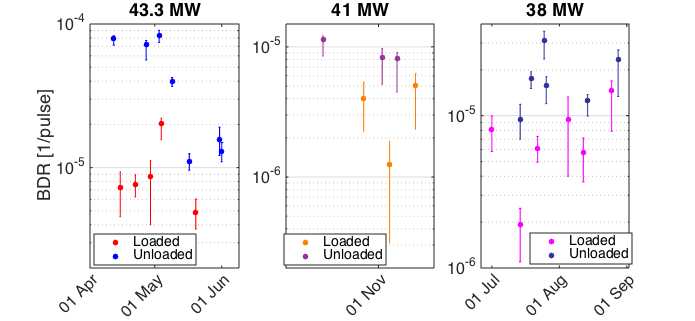
\includegraphics[scale=0.6]{pictures/BDR_zooms.png}
\caption{Comparison of the breakdown rate at different input power in three periods of stable running without switching input power.}
\label{BD_prob}
\end{figure}

It has to be noted that there are two exceptions to the last affirmation: the unloaded run at 43.3MW input power at the end of March (plotted in blue in Fig. \ref{BDR_history}), and the last loaded run of the year at 38 MW input power (see dedicated plot in Fig. \ref{BD_prob_last_raise}). 

In the first case, it is not clear why the BDR was that low, even it looks an anomaly considering the general trend of the precedent runs. It also has to be pointed out that the run is shorter than the others.

Regarding the second case, the BDR of the loaded and unloaded runs seems to converge at the end of the year. In addition, the last loaded run present a higher BDR than the precedent and following unloaded runs. Most likely this behaviour is addressable to a statistical fluctuation, but there is no way to know it because of the stop of the experiments for the end of the year.

\begin{figure}[h]
\centering 
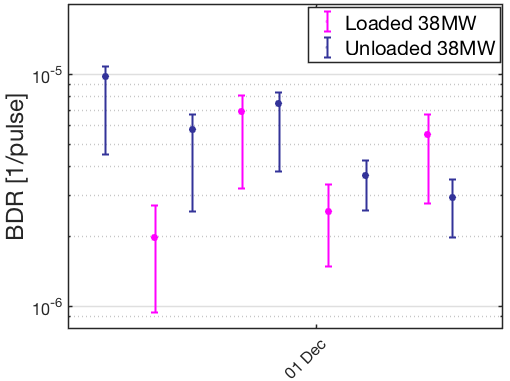
\includegraphics[scale=0.6]{pictures/BDR_last_part_year.png}
\caption{Measured breakdown rate at the end of the year}
\label{BD_prob_last_raise}
\end{figure}





\section[Breakdown distribution]{Breakdown distribution}

\subsection[A model for the breakdown distribution]{A model for the breakdown distribution}

Unloaded experiments exhibit a flat distribution of the breakdowns in the accelerating structure. In addition, it is known that the breakdown rate follows the scaling law in Eq. \ref{E30}, but it has been derived from the data available from the unloaded tests as well. From these considerations arises the necessity to understand if these results are still valid when running with the beam inside the accelerating cavity.

Considering any cell as a substructure, it is reasonable suppose that cells with a higher accelerating field will be more likely to experience breakdowns than cells with a lower field. According to this reasoning and following the Eq. \ref{E30}, the breakdown probability per cell is given by
\begin{equation}
\text{BD probability (\%)} =\frac{   \left ( \frac{E_\text{cell}}{E_\text{max}} \right )^{30} }{ \sum \left( \frac{E_\text{cell}}{E_\text{max}} \right )^{30}   }
\end{equation}
where E$_\text{cell}$ is the surface electric field in the centre of the cell and E$_\text{max}$ is the maximum surface electric field at the centre of a cell. 

The choice of using the surface electric field instead of the accelerating gradient comes from the physics of the breakdown process \cite{Walter:PC}. Anyway the shape of the gradient profile and of the surface electric field along the structure differs only slightly. The field of the coupling cells is assumed as the same in the adjacent cells. This comes from geometrical considerations, and could be eventually derived from simulations \cite{Alexej:PC}.

The result is shown in Fig. \ref{BD_prob}. The expectation is to have a almost flat distribution in the unloaded case, with and accumulation of the number of breakdowns in the first part of the structure for the loaded case and at the end of the structure for the antiloaded case.


\begin{figure}[h]
\centering 
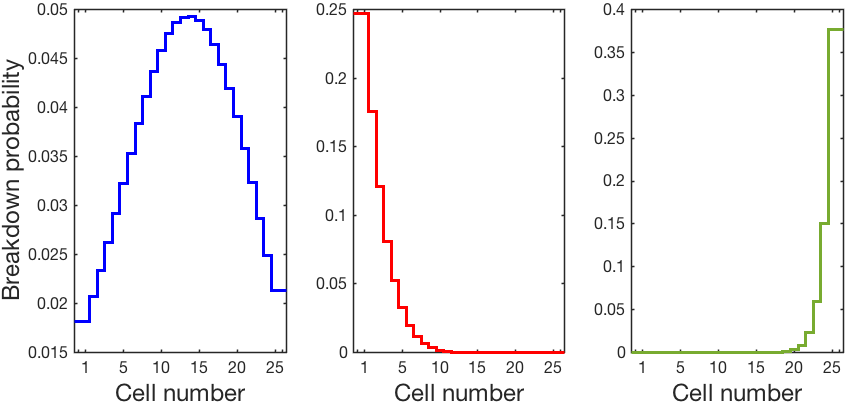
\includegraphics[scale=0.45]{pictures/BD_probability.png}
\caption{Breakdown probability according to the model in different running conditions: unloaded (left), loaded (center), antiloaded (right). The different scale has to be noted: while the breakdown probability oscillates between the 1.8\% and 5\% in the unloaded case, when the beam is present the difference is much bigger.}
\label{BD_prob}
\end{figure}


\subsection[Measurement results]{Measurement results}

The breakdown distribution, cumulating the data at the same input power, are shown in Fig. \ref{BD_distro}. Both the linear scaling with the surface field and the scaling proposed in the precedent section are plotted.

In the centre of the structure there is a warmer part, where are happening a large number of breakdowns. This warm region is present both in the unloaded and loaded runs, and could be provoked by: 
\begin{enumerate}
\item the development of an hotcell
\item surface damage of the central cells, where for some reason the surface is rougher and provokes more breakdowns. 
\item a particular pattern coming from the design of the structure
\end{enumerate}
Fortunately, there is no sign of the development of an hotcell. Figure \ref{BD_3d} shows that although a warmer region in the centre developed after the antiloaded runs in June 2016, it was gradually reconditioned during the following part of the year. 

It is not possible to decide between the second and third option for the moment. Additional hints will come from the post-mortem analysis of the structure, that will be cut and examined with various microscopy techniques. This analysis will take place later in 2017. In any case, the second option looks the most probable. 

The breakdown distribution is compatible with a constant distribution during runs without beam. It is also compatible with the hypothesis of accumulation of the breakdowns in  the first part of the structure during the loaded runs and at the end during the antiloaded runs.

The fundamental result from this is anyway that the breakdown probability is ruled by the peak accelerating gradient, and not from the average accelerating gradient.


Even ignoring the central warm zone, it is not clear which law rules the distribution of the breakdowns in the cells. Collecting more data is necessary for this purpose.

\begin{figure}[h]
\centering 
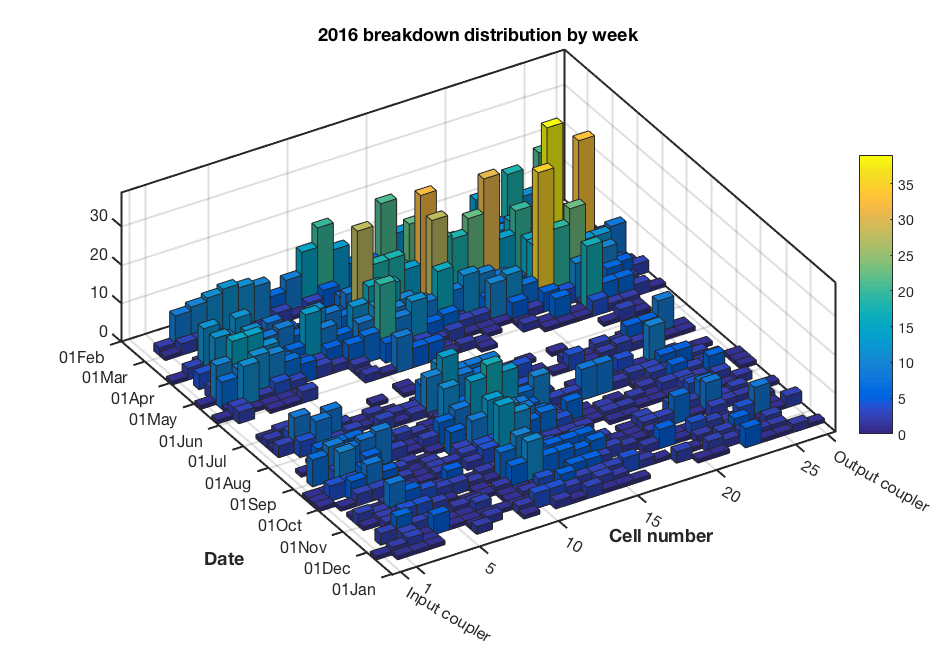
\includegraphics[scale=0.4]{pictures/week_distr_3D.png}
\caption{Breakdown number per cell per week. }
\label{BD_3d}
\end{figure}



\begin{landscape}

\begin{figure}[h]
\centering 
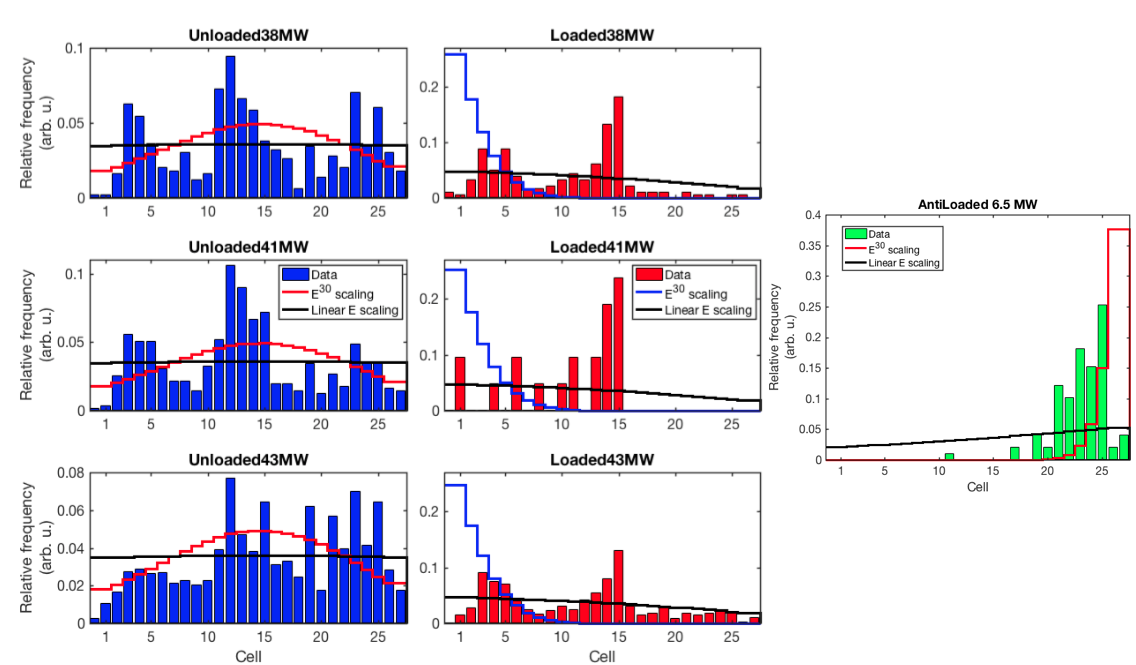
\includegraphics[scale=0.53]{pictures/distro_all.png}
\caption{Measured breakdown distribution in the accelerating cavity under test in different running conditions. Over the data is plotted the proposed scaling and the linear scaling with the surface field is plotted (in black).}
\label{BD_distro}
\end{figure}
 
\end{landscape}





\section[Beam induced RF]{Beam induced RF}

The effect of the beam is observable on the RF signals after a breakdown. Figure \ref{BI_rf_fig}  shows two examples of RF signals. Three moments are clearly visible in the transmitted power signal: the power falls after the breakdown; the beam start producing power in the accelerating cavity, which is not filled anymore with the RF downstream the breakdown; the power production stabilises with the establishment of a plateau. 

In the figure two different examples are presented. On the right it is visible the spike, but the plateau does not have time to develop because of the end of the beam pulse. On the left the full development of the process is appreciable.

\begin{figure}[h]
\centering
  \subfigure[Breakdown happening early in the pulse]
   {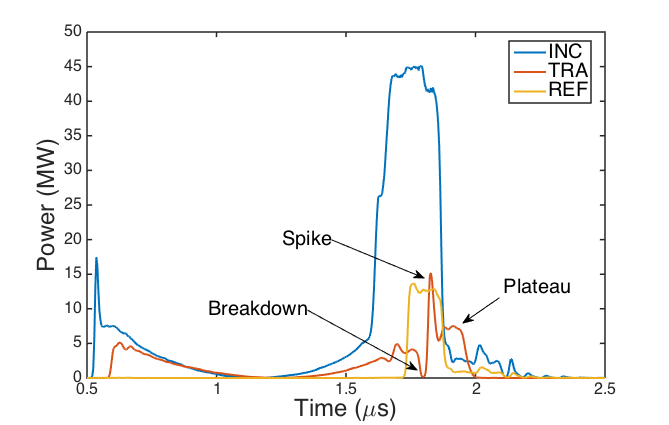
\includegraphics[scale=0.33]{pictures/BI_rf.png}}
   \hspace{2mm}
  \subfigure[Breakdown happening late in the pulse]
   {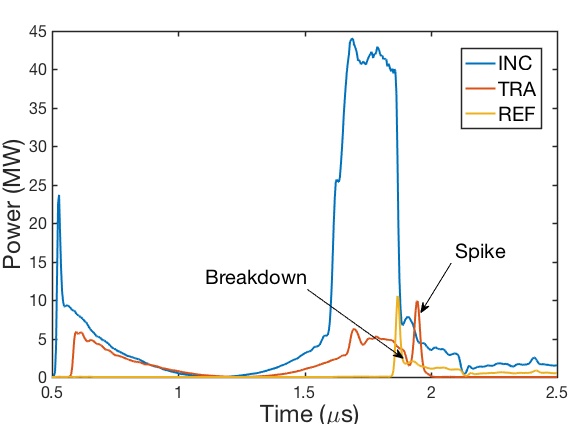
\includegraphics[scale=0.33]{pictures/BI_rf_2.png}}
\caption{Two examples of RF signals for a breakdown event earlier and later in the pulse. In both case the spike provoked by the beam-induced RF production is visible. In the early case (a) it is possible to see the development of the plateau induced by the stabilisation of the power production up to the end of the beam pulse. In the late case (b) the beam pulse duration is not enough to allow the development of a stable condition.}
 \label{BI_rf_fig}
 \end{figure}


\section{Conclusions}

The experiment described in this work offers a first glimpse on the beam effect on the breakdown rate in a normal-conducting travelling-wave accelerating structure.

During the 2016 measurement campaign, the expertise to realise breakdown experiments with the beam has been gained. The experiment were conduced with a longer beam pulse and with higher current than the CLIC Main Beam parameters to enhance the effect of the beam on the BDR.

This work showed that the breakdown rate is in general lower during experiments with the beam, conduced with the same input power. 

The distribution of the breakdowns in the accelerating cavity is compatible with the accumulation of the breakdowns in the front part of the structure when accelerating the beam and in the last part when decelerating. This behaviour support the dependence of the local breakdown probability from the local surface field. Unfortunately, the development of a warm zone in the centre of the structure makes impossible to find the scaling law for the breakdown distribution. 

An enhanced migration of the breakdowns have been detected during the loaded runs. This result agrees with the modified field profile induced by the loading of the cavity with the beam.

Further investigations in this field require to repeat the experiment in stable conditions, with measurements of long duration (weeks). This last request translates into long beam times that the tight scientific program of the CTF3 was not able to support. Missing this condition, it is not possible to understand if the continuous switching between different running conditions impacts on the fluctuation of the breakdown rate. Anyway it is reasonable to expect that this causes a higher breakdown rate than the one achievable running in stable conditions. 

The experiment has to be considered successful, because of the amount of informations that have been collected, even with a limited and not continuous beam time in a non-dedicated experiment.



\section[Further developments]{Further developments}

The experience gained from this work allows first of all to suggest some modifications to the setup, starting by looking at the newer Xboxes:
\begin{itemize}
\item The substitution of the TWT with a solid state amplifier will avoid the presence of spikes. The new amplifier has been installed in XBOX1 at the beginning of 2017.
\item Switching the pulse compressor from SLED-I to SLED-II type (as is in Xbox2), and place the Xbox closer to the structure under test would solve the detuning problem (since the attenuation of the waveguides is lower and the power requested to the pulse compressor as well).
\item The missing back-off of power has to be investigated and solved. Probably the performance of the interlock system program running on the FPGA could be improved by writing the related code in a hardware description language instead than LabVIEW.
\item The sampling rate of the log detectors could be improved up to 1 GSa/s using the same acquisition system used for the IQ detectors.
\end{itemize}

On the physics side, pursuing the experiments in a dedicated facility would be the optimal solution. As general guideline, alternating three weeks of experiments with beam to three weeks of unloaded experiments could be a good programme. This would allow to get more meaningful results and compare with the unloaded results of the Xboxes, where the normal experimental time is weeks.

Beyond the physics interest, before the implementation of CLIC, a simulation of the CLIC operation would be very interesting. In this context, the comparison of the operation of the cavity at 100 MV/m average gradient would be extremely interesting.